
\chapter*{Chapter \ref{chapter:nat} Supplementary Information}
\chaptermark{Chapter \ref{chapter:nat} Supplementary Information}
\addcontentsline{toc}{chapter}{Chapter \ref{chapter:nat} Supplementary Information}

\noindent\emph{Note: The `main manuscript' referenced in this supplement refers to Chapter~\ref{chapter:nat}. As such, `figure 1 of the main manuscript', for example, refers to figure \ref{chapter:nat}.1.}


\section*{Materials and Methods}


\subsection*{Experimental Setup}

Two computers were used for this experiment: One to display the stimuli and another to record EEG. Stimuli were shown on an Iiyama ProLite B2776HDS 27$''$ display using a resolution of 1920$\times$1080 pixels, located approximately one meter away from the participants. The keyboard used was a standard US layout computer keyboard.

EEG was recorded continuously using 64 active Ag/AgCl electrodes (actiCAP; Brain Products GmbH, Munich) mounted according to the extended 10-20 system on an elastic cap (EASYCAP GmbH, Munich). The signal was sampled at 500 Hz and amplified using BrainAmp DC amplifiers (Brain Products GmbH, Munich). All electrodes were referenced to FCz and the ground electrode was placed at AFz.

EEG data was recorded and combined with the paradigm's markers using the Lab Streaming Layer framework (Swartz Center for Computational Neuroscience [SCCN], University of California, San Diego [UCSD]).


\subsection*{Experimental Paradigm}

The cursor's movements were restricted by the nodes of a visible grid. The cursor started out on one of these nodes and, for each movement, could only move to one of the adjacent nodes. Depending on the cursor's position in the grid, then, there were up to eight possibilities for one movement. The grid consisted of gray open circles connected by gray lines on a black background. The cursor in this paradigm was a red, filled circle. The cursor's size was 4.5\% of the display's total height, the grid nodes' size 6\%, and the horizontal and vertical grid lines' length 15\%. Line thickness between the grid nodes was set to 2 pixels. `Red' was pure \textsc{RGB}(255,0,0), `gray' \textsc{RGB}(51,51,51) and `black' \textsc{RGB}(0,0,0). The dimensions of the grid are discussed below.

An animation allowed the participants to be able to anticipate the moment of each movement. Over the course of one second, a white `ghost cursor' would grow inside of the actual cursor. As soon as this ghost reached the same size as the actual cursor, it would instantaneously be repositioned to the chosen adjacent node, while also highlighting the grid line connecting the two nodes in white. `White' here was pure \textsc{RGB}(255,255,255), and the highlighted grid line's thickness was increased to 3 pixels. The movement remained visible for one second, with the red original cursor still on the initial node, the white ghost cursor on the new node, and a white line connecting them. Following that, all whites disappeared and the (red) cursor would instantaneously move to and remain at its new position, on the new node, for another second, before the animation would start over for the next movement. In all, a single trial was three seconds in length.

Grids of three different dimensions were used in this study: One by three nodes ($1\times3$), four by four nodes ($4\times4$), and six by six nodes ($6\times6$).

On each grid, a single red node in one of the corners indicated the current target. Once the cursor had landed on this target node, a new grid was started with the same dimensions, but a different layout. For the $1\times3$ grids, each new grid was rotated either 45, 90, or 135 degrees relative to its predecessor, and a new target corner was chosen at random (`corner' here is one of the two ending nodes of the grid row). The larger grids did not rotate, but a new target was selected for each new grid such that no two subsequent grids had a target in the same corner. Each newly started grid was displayed for one second before the first movement was initiated, for the participants to orient themselves.

In all grids, the cursor's starting position was one node away from the corner opposite the target's, in a straight line to the target. 

Supplementary Figure S1 illustrates the stimuli; Supplementary Movie S4 contains animated stimuli as seen by the participant.

For each individual cursor movement, a movement direction was chosen randomly from the set of possible movements. By default, all possible directions had an equal probability of being selected, and during the offline (calibration) sessions, these initial probabilities remained unchanged---the cursor was unbiased and moved randomly. However, during online application of the pBCI, the directional probabilities were altered based on the classification of each movement as either `correct' or `incorrect', biasing the cursor to repeat movements classified as `correct'.

Specifically, all movement directions were represented a specific number of times in the set from which each new movement was randomly selected. After classification, the respective directions' numbers were increased or decreased such that the resulting probability of each subsequent direction is given by

\begin{displaymath}
    p=\frac{mx}{n+(m-1)x}
\end{displaymath}

\noindent where $x$ is the respective direction's initial number of shares in the set, $n$ is the full set's initial size, and $m$ is a multiplier. For a movement classified as `correct', $m$ was 2.0 for that movement's direction and 1.5 for the two adjacent directions; for movements classified as `incorrect', $m$ was 0.5 and 0.75, respectively. All directions started with a share of 100 elements each in the set. All shares below 1 were rounded up at the time of selection.

The adaptation of adjacent directions represents a certain degree of leniency which the participants were assumed to show in their judgements: If the target is a few nodes north of the cursor's current position, a first move to the north-west is imperfect but may still be acceptable. Therefore, the feedback received from a movement to the north-west should not only alter this specific direction's probability, but should also influence subsequent movements to both the north and the west. 

All visible on-screen events were marked in the EEG stream and additional information about each cursor movement was logged, including distance to the target and the movement's direction relative to the target direction (i.e., a straight line unconstrained by the grid represented a 0$^\circ$ movement).

The paradigm was written in Python using the Simulation and Neuroscience Application Platform 1.02-beta (SCCN, UCSD; https://github.com/sccn/SNAP).


\subsection*{Participants}

A total of nineteen participants participated in this study, with an average age of 25.4 years $\pm~3.4$. Seven were female, and a total of two participants were left-handed. Participants were asked, alternately, to use either their left or their right hand to indicate their judgements. This resulted in ten participants not using their dominant hand. All had normal or corrected to normal vision. Instructions were given in writing, in German. While all knew German, thirteen did not have German as their mother tongue; these were verbally given additional, standardized instructions. 

Nineteen participants performed calibration trials, while sixteen of them additionally performed online trials.


\subsection*{Experimental Procedure}

All participants were informed of the nature of the experiment and the recording and anonymization procedures before signing a consent form. The ethics committee of the Department of Psychology and Ergonomics at the Technische Universität Berlin approved the experiment and the procedures.

After preparation and setting up the EEG cap, which took roughly one hour per participant, participants were seated in a padded chair in a dimly lit room, about one meter away from the stimulus display. In writing, they were instructed to judge each individual cursor movement on the display as either `acceptable' or `not acceptable', with respect to reaching the target, and to indicate their judgement by pressing either `v' or `b', respectively, on a computer keyboard using one and the same finger of one hand. The participants performed this task during all blocks. 

Participants were first given four blocks of 50 trials on $1\times3$ grids. Here, the cursor performed only one movement per grid: Regardless of whether or not that movement reached the target, a new grid was subsequently started. This was because after a movement away from the target, only one movement possibility would remain, i.e. that trial would have no informational value. Breaks between these blocks were self-paced, and participants were given time to practice before the first block was started. 

Following these first blocks, participants received additional instructions for the larger grids, emphasizing their task to judge every movement individually and independently of the cursor's movement history. Participants were again given some time to practice, on a $4\times4$ grid, and then performed five blocks of 120 trials on grids of that size. Here, if the target had not been reached after 55 trials in one grid, a new grid was started. 55 is twice the median number of random movements required to reach a target on a $4\times4$ grid.

Taking symmetry and rotation into account, a total of 43 unique cursor movements are possible on the $4\times4$ grid, i.e., 43 unique pairs of distance and angular deviance. In between the five calibration blocks, in four sessions, participants were shown, in random order, all 43 unique cursor movements. For each of these, participants were asked to rate it as either `acceptable' or `not acceptable', and on a scale of 1 to 5, with 5 being `the best possible movement in that situation', and 1 being `the worst'. Here, unlike during the blocks, there was no time limit imposed on their answers.

EEG recorded during these latter five blocks served to calibrate the classifier, as discussed in \emph{Feature Extraction and Classification}. This classifier was then applied to one more block of 120 trials on $4\times4$ grids, and one last block of 120 trials on $6\times6$ grids. No maximum number of trials other than the block's length was set for these online blocks. 


\subsection*{Feature Extraction and Classification}

A BCI based on supervised machine learning needs to be calibrated before it can be applied. This calibration is typically performed on sets of recordings, usually EEG epochs, which are known to contain the signals that need to be detected later. On the basis of these epochs, a classifier is calibrated to optimally distinguish between the different classes of source signals.

The classes the classifier was calibrated on were formed on the basis of the movements' angular deviance from a straight line towards the target, as illustrated in Supplementary Figure S2. `Correct' movements were those with an absolute angular deviance of 0$^\circ$; `incorrect' were those with an absolute angular deviance of 135$^\circ$ or more, as in Supplementary Figure S3. These class definitions were determined based on the first three participants' data.

Note that the participants' judgements, indicated using button-presses, were ignored: Only a movement's angle with respect to the target determined its class. Movements between 0 and 135$^\circ$ were not included for calibration.

The open-source toolbox BCILAB \cite{kothe2013bcilab} version 1.01 was used to define and implement the pBCI. This approach extracted features from the time course of each of the 64 channels by subsampling the ERPs of each epoch. This was done by dividing the time course into a sequence of 8 consecutive 50 ms windows (8 time windows starting at 50 ms after cursor movement) and replacing each window by its average. The resulting features were thus one value for each channel in each time window. Linear discriminant analysis (LDA) was then applied to these features generated from all available calibration trials to distinguish between the features belonging to the two classes. The outcome of the LDA is a linear weighting of all features. In other words, in each time window all channels receive a weight according to their relevance for classification in that specific time window. The linear combination of all features of one single trial with these weights then gives a number between -1 and 1, indicating whether this trial is classified as belonging to class 1 or to class 2.

For the feature extraction, the data was first resampled at 100 Hz, and band-pass filtered from 0.1 to 15 Hz. Linear discriminant analysis was regularized by shrinkage. A [5,5]-times nested cross-validation with margins of 5, ensuring the independence and identicality of the feature distributions, was used to select the shrinkage regularization parameter, and to generate estimates of the model's online reliability. 



\subsection*{Extended Feature Analysis}

The method used by the pBCI to extract discriminative information (described in \emph{Feature Extraction and Classification}, above) can be analyzed to reveal further insights into the relevant underlying processes. The classification model used here is a multivariate approach, a linear discriminant analysis (LDA), optimized for the discriminability of the extracted features between classes. Each feature represents data at a single sensor for one of the chosen time windows. Hence, the methodology recently introduced by \citeA{haufe2014} could be applied to interpret the classification model.

For one of the eight 50~ms time windows, Figure 2 in the main manuscript illustrates three aspects of the information used by the pBCI: its scalp topography, its estimated source within the brain, and the activity of that source as filtered from the EEG, i.e. the selected signal of interest.


\paragraph{Signal of interest} Panel \emph{c} of Figure 1 in the main manuscript shows the EEG activity projected by the LDA filter for the third time window, i.e., the combined activity of all 64 channels as filtered by the classifier. Supplementary Figure~S5 illustrates this for all eight time windows.

In Supplementary Figure~S5, the ERP is shown for eight groups of cursor movements, time-locked to that movement, as well as the difference wave between the two classes (`correct' and `incorrect'). The difference wave represents the actual signal (and the optimization target) used by the classifier, in the corresponding time window. The time window of the LDA filter used is indicated in gray.

Each figure indicates the response to different cursor movements of those processes whose activity was filtered from the EEG in that time window, over the course of a full second. 


\paragraph{Identifying scalp projections} In panel \emph{a} of Figure 1 in the main manuscript, the scalp map shows, on average for all participants, the (interpolated) activation pattern which illustrates how the signal of interest is expressed in the 64 channels \cite{haufe2014}, in the third time window. Supplementary Movie S1 shows this activation pattern over the full length of the used 400 ms.

For each participant, LDA patterns $A = (a_{j})_{j}$ were generated from the LDA filters $M = (m_{j})_{j}$ originally used for online classification by conjugation with the features' covariance matrix $C$: $A = CMC^{-1}$. Spatial interpretation of these patterns for each time window reflects a mixture of scalp activations related to discriminative source activity $\widehat{A} = (\widehat{a}_{j})_{j}$ and class-invariant noise representation $N$, with $A = \widehat{A} + N$. An estimate of $\widehat{A}$ can be generated by reducing the filter entries representing class-invariant noise by weighting each filter entry $m_{j}$ with the correlation of its associated feature activity vector over trials $F_j$ to the binary vector of true class labels $L$: $$\widehat{m}_{j} = corr(F_j,L)*m_{j}$$ Conjugating the resulting correlated filters $\widehat{M} = (\widehat{m}_{j})_{j}$ with $C$ gives the resulting correlated pattern $\widehat{A} = (\widehat{a}_j)_j$. $\widehat{A}$ can be visualized by topographic plots for each time window identifying the scalp projections of the most discriminant source activity at that time, as in Figure 1 of the main manuscript and Supplementary Figure S5, and Supplementary Movie S1. \\


\paragraph{Identifying relevant sources}
To identify the sources underlying these topographic representations, the backward model, i.e. the LDA filter, was combined with an independent component analysis (ICA). The ICA unmixing matrix $W=(I_1,I_2,\cdots,I_n)$ was determined on previously manually cleaned data for each participant by using the Adaptive Mixture ICA (AMICA) Toolbox \cite{palmer2012amica}, such that $s = Wx$, where $s$ represents the source activation related to a given scalp activation $x$. For each time window, the relevance for classification $R_i$ of each independent component $I_i$ can then be determined by distributing the LDA filter weights to the independent components via $W$, weighted by two factors. The first factor is compensating for the amplitude alignment of the LDA filter weights to the feature amplitudes. It is determined by calculating the variance over trials of the feature $\widehat{F}_i$ extracted from the time series of the independent component: $V_i = var(\widehat{F}_i)$. A second weight is determined for filtering out noise representations by weighting the independent components with the correlation of their feature activity to the true class labels (as described above for electrode activity). $$ R_i = V_i * corr(\widehat{F}_i,L) * W M $$ \\


\paragraph{Localizing relevant sources}
To localize the identified sources, equivalent dipole models that describe the most likely position of the source in a standard head model were identified for selected components by using the EEGLAB plug-in DIPFIT 2.x \cite{oostenveld2003dipfit}. Components were selected by a threshold criterion for residual variance of the dipole model ($RV < 0.15$) and visual inspection of activation spectra, time courses, and scalp topographies. Only components reflecting cortical, ocular, or muscular activity were included in the analysis.

For each time window, each of the 371 resulting dipoles was weighted by the relevance $R_i$ of its associated independent component, described above. The areas of high relevance were then described by a weighted dipole density plot using the EEGLAB plug-in dipoleDensity \cite{miyakoshi2013dipdens}. 

Supplementary Movie S2 shows the result of this analysis over the full length of the used 400 ms, by plotting the dipole density per cubic millimeter weighted by the relevance $R_i$ of each included dipole with a smoothing kernel of 12~mm.

The above-mentioned process of selection did not markedly influence this analysis. Compared to all 1191 dipoles and averaged over the eight time windows, the 820 rejected dipoles (68.85\%) carried 7.5\% of the weights distributed by the classifier. Relative to all 1191 dipoles, a total of 87 dipoles received a relevance weight larger than 1 standard deviation in at least one of the time windows. These 7.3\% of dipoles carried 77.82\% of all total weight distributed by the classifier. Four of these highly weighted dipoles (4.6\%) were rejected in the process explained above and not included in the analysis. These four represent 1.67\% of the weight included in the analysis. Three belonged to the same subject.

\paragraph{Behavioral analysis}
Participants indicated their evaluation of each movement as `acceptable' or `not acceptable' through button presses. A paired-samples t-test was conducted to compare the subjects' mean reaction times. There was a significant difference between `acceptable' button presses (mean 369.7 ms±66.9) and `not acceptable' button presses (mean 310.7 ms ±60.7); t(18) = 8.347, p<0.001. This calculation included only reaction times between 100 and 1000 ms.

No systematic effect reflecting this delay can be found in the ERPs used for classification however see Figure 1, and Supplementary Figure S5). This, in combination with an absence of relevance weights in the motor cortex (Supplementary Figure S5) and the ERPs' independence of eye movements (Supplementary Figure S6), leads us to conclude that the behavioral delay has had no effect on the passive BCI.  


\subsection*{Performance Measures and Statistics}

The performance of the cursor was operationalized as the number of movements required to reach the target. Trials at the end of a block that did not contribute to reaching a target or hitting the maximum number of trials for that attempt, were discarded. This measure does include those attempts that hit the maximum number of trials, which happened a total of seven times to seven participants on the 4$\times$4 grid, and to two participants on the 6$\times$6 grid. This resulted in 88 pBCI-supported data points for the 4$\times$4 grid, and 47 for the 6$\times$6 grid. 

As a comparison, a sample of around 7000 data points was taken using the same measure from non-supported (random) blocks. This data is non-parametric and varies greatly. Therefore, a resampling approach was taken where the available sample of pBCI-supported measures was repeatedly compared to a new random sample of the same size of non-supported performance measures. This comparison was done through a Wilcoxon rank-sum test. Out of 50 000 such comparisons, 98.02\% of tests were significant at the $\alpha=0.025$ level for the 4$\times$4 grid performance measures; for the 6$\times$6 grid, 100.00\% of tests were significant at this level. On a 4$\times$4 grid, non-supported cursor movement required on average (median) 27 trials to reach a target, whereas with BCI support, this decreased to an average of 13. On a 6$\times$6 grid, the median values were 90 and 23, respectively. 

The pBCI-supported performance was furthermore compared to `perfectly supported' performance, where the cursor was reinforced as during the online sessions, except automatically, with perfect accuracy. Here, all movements with an angular deviance less than 45º were judged to be `correct' and reinforced accordingly, and all others were `incorrect', and their probabilities decreased as described in Supplementary Method 2. The same procedure as above yielded significant differences to the pBCI-supported measures for both the 4$\times$4 grid (99.98\% of tests at $\alpha=0.025$) and the 6$\times$6 grid (100\%). The median perfectly supported performance measure on the 4$\times$4 grid is 10 movements, and 14 movements on the 6$\times$6 grid.

Additionally, the mean directional probabilities upon reaching the target in both online grids (combined) were calculated. These are illustrated in Supplementary Figure S4. Supplementary Table S2 lists the Bonferroni-adjusted results of pairwise post hoc tests from a one-way ANOVA (F(7,105)=57.520, p<0.001) on this data. On average, the classifier has been able to reinforce the `correct' directions significantly more strongly than `incorrect' directions.



\subsection*{Linear Dependency of Peak Amplitude}
Figure 1 of the main manuscript shows a linear scaling of peak amplitudes with respect to absolute angular deviance away from the target, projected by the filter weights of the third time window. The eight groups of angular deviations were selected such that for each single participant, at least 50 trials were present in each group, i.e., for an optimal signal to noise ratio while maintaining maximal angular resolution. 

Figure 1 shows the same linear scaling in the grand average ERP ($n=19$) at Fz. This ERP has been further investigated using standard neurophysiological methodology.

For the derivation of the single electrode ERP, BrainVision Analyzer was used\footnote{Version 2.0.2.5859, Brain Products GmbH, Munich, 2012}. The raw EEG data was first band-pass filtered from 0.5 to 45 Hz, and decomposed into statistically maximally independent source signals through ICA. Individual components that resembled eye movements and eye blinks were manually selected for removal based on their time course and topography \cite<e.g.,>{jung2001}. Figure 1 shows the grand average ERP over all nineteen participants at Fz with these components removed. For a comparison, Supplementary Figure S6 shows the grand average ERP at Fp1, Fp2, and Fz for only the removed components. No systematic response is visible, pointing to cortical causes of the differences. At Fz, where the cortical components peak around $+3.9\mu$V for e.g. the $0^\circ$ condition, the eye components show an amplitude of $-0.37\mu$V.

Statistical analysis focused on the systematic peak differences seen at Fz around 180 ms. A one-way ANOVA indicated a significant influence of angular deviance on peak amplitude ($F(7,126) = 47.243, p < 0.001$). Post-hoc comparisons corrected for false discovery rate are listed in Supplementary Table S3 and illustrated in Supplementary Figure S7. The peak amplitudes differ significantly ($p < 0.001$) between the classes used by the classifier. In between, the peak amplitudes scale linearly with angular deviance, as fitted by a linear regression model using each group's mean angular deviance as predictor ($b = -0.0035, F = 45.28, p < 0.001; R2 = 0.33$). Classifier output followed a similar trend, as in Figure 1 of the manuscript. 

\begin{figure}[p]
    \renewcommand\thefigure{\ref{chapter:nat}.S1}
    \centering
    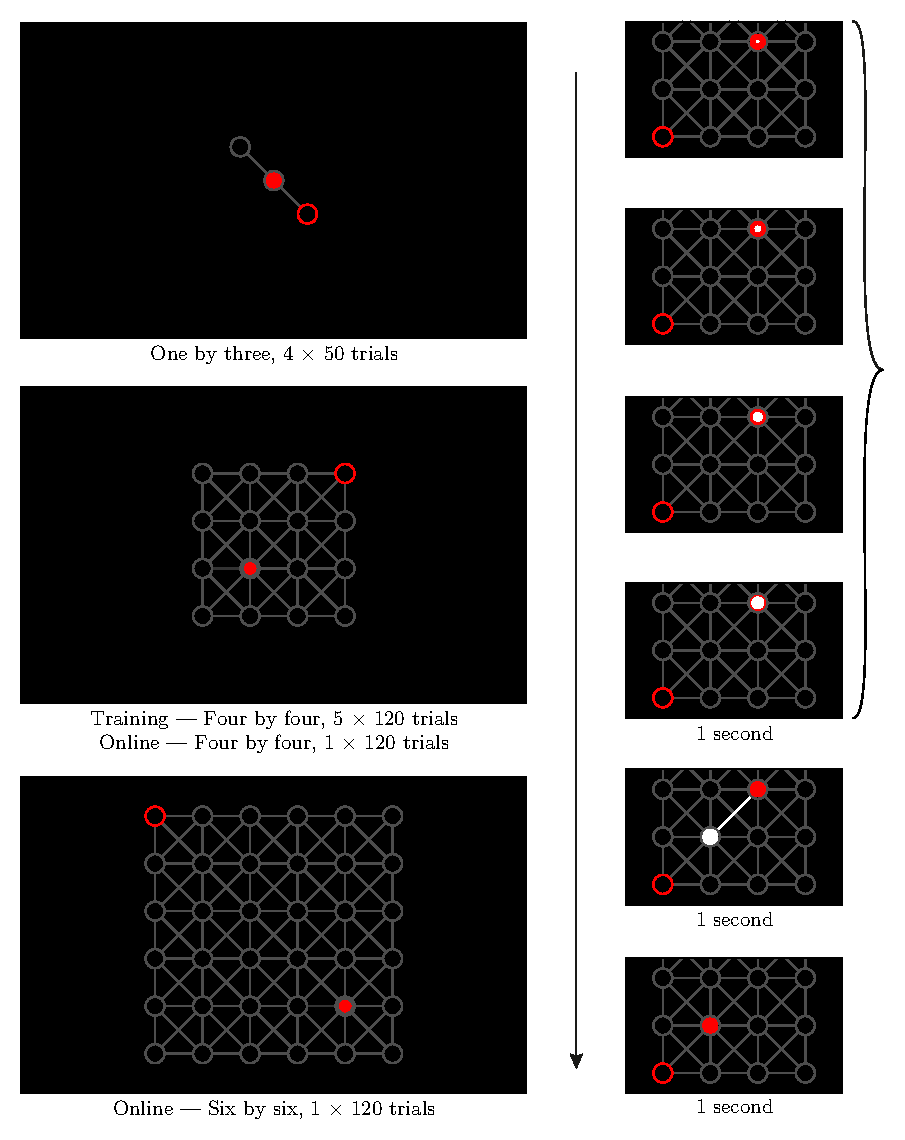
\includegraphics[width=\textwidth]{figures/nat-app-fig-s1.pdf}
    \caption[Experimental paradigm and procedure.]{Experimental Paradigm and Procedure. The experimental paradigm and procedure. \textit{Left}: Three different grid sizes were used in the experiment. Data from five blocks in 4$\times$4 grids was used to calibrate the classifier, which was then applied to another 4$\times$4 block, and one block on a 6$\times$6 grid. Data from the 1$\times$3 grids has not been used in this paper. Each cursor movement consisted of the cursor moving from one node to one of the directly adjacent ones. The cursor could move horizontally, vertically, and diagonally over the grid. Since the target was known and indicated, for each movement, it was possible to determine a measure of correctness for each movement by means of calculating the angular deviance, as in Supplementary Figure S2. \textit{Right}: Detail of a 4$\times$4 grid showing the cursor's movement animation.}
\end{figure}

\begin{figure}[t]
    \renewcommand\thefigure{\ref{chapter:nat}.S2}
    \centering
    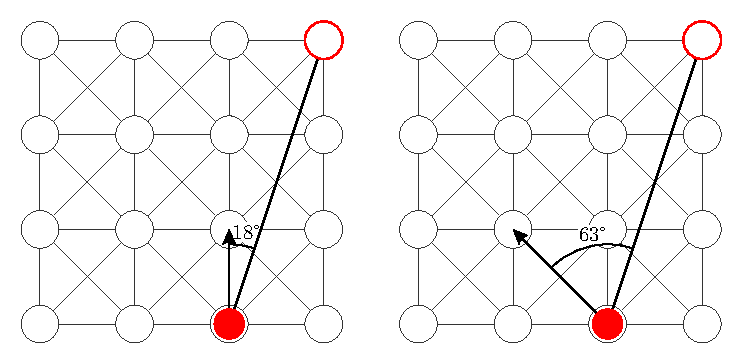
\includegraphics[scale=1.25]{figures/nat-app-fig-s2.pdf}
    \caption[Angular deviance.]{Angular Deviance. Illustration of the angular deviance of two possible cursor movements (north, and north-west) from the optimal path straight towards the target. Angular deviance was measured as the absolute deviation, in degrees, of the movement direction from a straight line to the target.}
\end{figure}

\begin{figure}[b]
    \renewcommand\thefigure{\ref{chapter:nat}.S3}
    \centering
    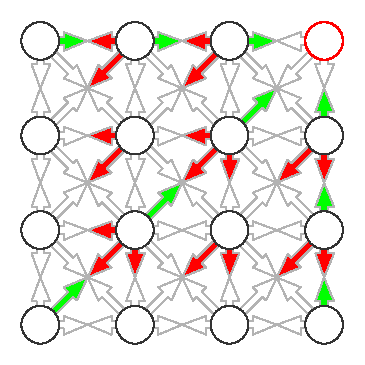
\includegraphics[scale=1.25]{figures/nat-app-fig-s3.pdf}
    \caption[Class definitions of the classifier's training set.]{Class Definition of the Classifier's Training Set. The classifier was calibrated on a subset of trials from a 600-trial calibration session. This set was selected by angular deviance: Movements with an absolute angular deviance to the target of 0º were included as `correct', while movements with a deviance of 135º or more were included as `incorrect'. This figure illustrates which of all possible movements on the 4$\times$4 grid were included, and in which category: Green represents `correct', red `incorrect'. From the total of 600 trials per participant on the 4$\times$4 grids, this selection left 62.7 ± 7.8 `correct' and 124.4 ± 8.9 `not accepable' trials per participant for the classifier to be calibrated on.}
\end{figure}

\begin{figure}[p]
    \renewcommand\thefigure{\ref{chapter:nat}.S4}
    \centering
    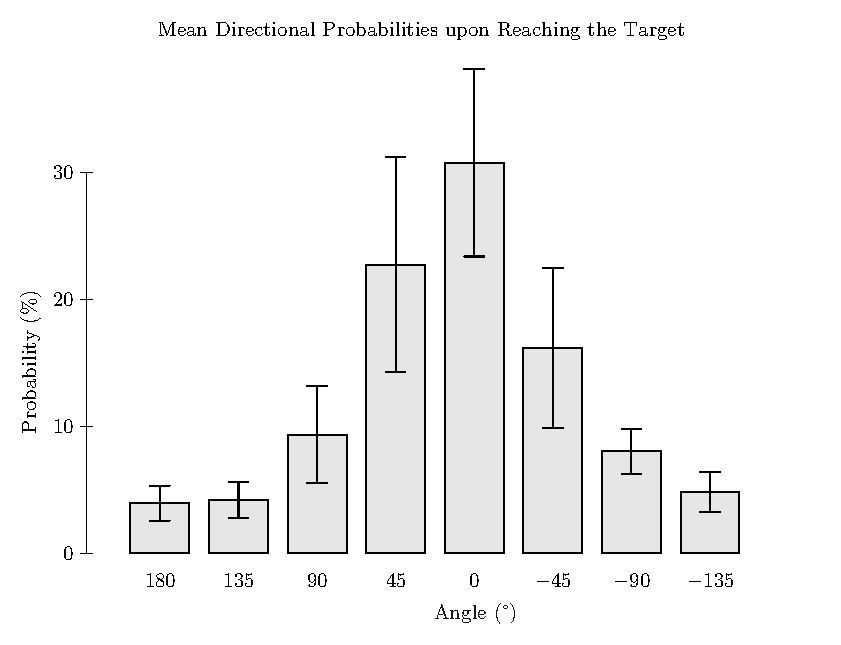
\includegraphics[width=\textwidth]{figures/nat-app-fig-s4.pdf}
    \caption[Mean directional probabilities upon hitting the target.]{Directional Probabilities. Mean directional probabilities, relative to the target from the cursor's starting position, upon hitting the target, in the BCI-supported condition, averaged over participants. Error bars represent the standard deviation. See Supplementary Table S2 for significance tests.}
\end{figure}

\begin{figure}[p]
    \renewcommand\thefigure{\ref{chapter:nat}.S5.1}
    \centering
    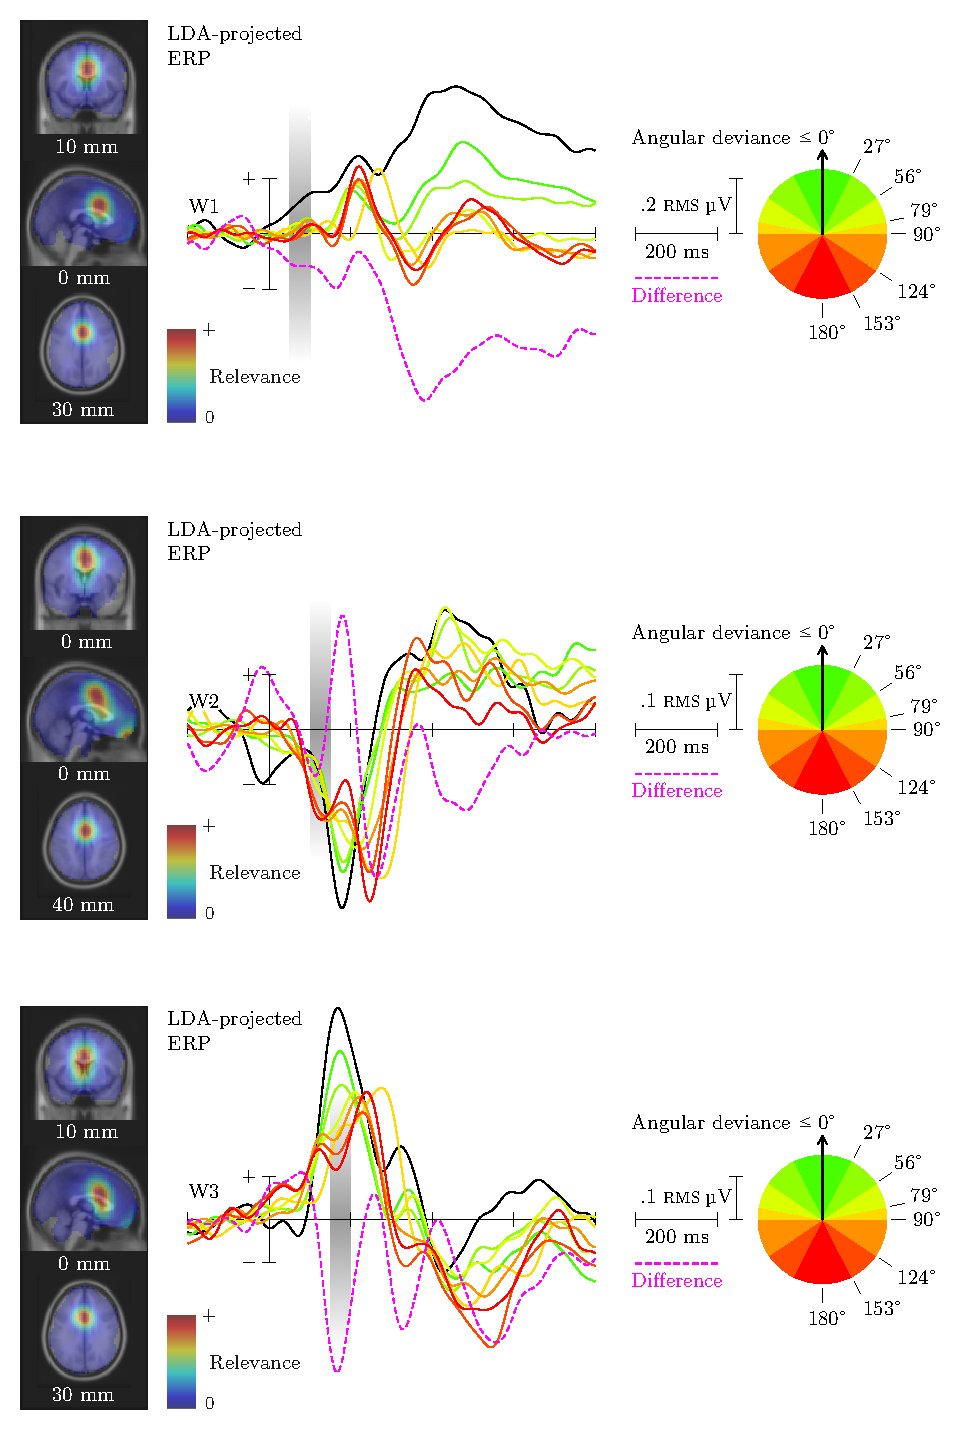
\includegraphics[width=\textwidth]{figures/nat-app-fig-s5-1.pdf}
    \caption{LDA-projected ERPs. (This figure spans three pages; this is page 1 of 3.)}
\end{figure}

\begin{figure}[p]
    \renewcommand\thefigure{\ref{chapter:nat}.S5.2}
    \centering
    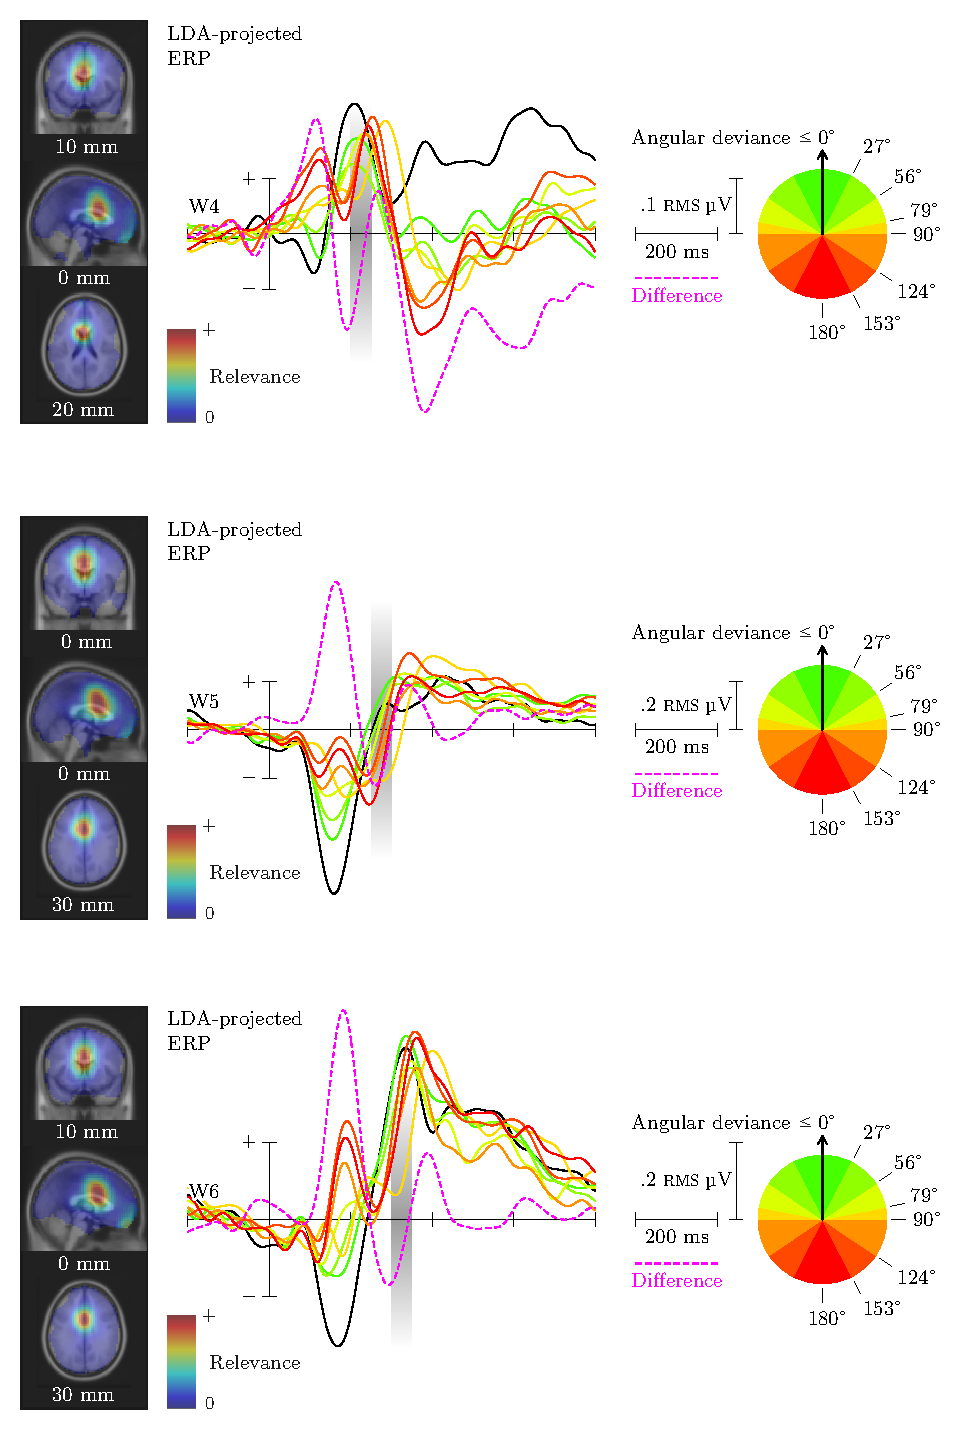
\includegraphics[width=\textwidth]{figures/nat-app-fig-s5-2.pdf}
    \caption{LDA-projected ERPs. (This figure spans three pages; this is page 1 of 3.)}
\end{figure}

\begin{figure}[p]
    \renewcommand\thefigure{\ref{chapter:nat}.S5.3}
    \centering
    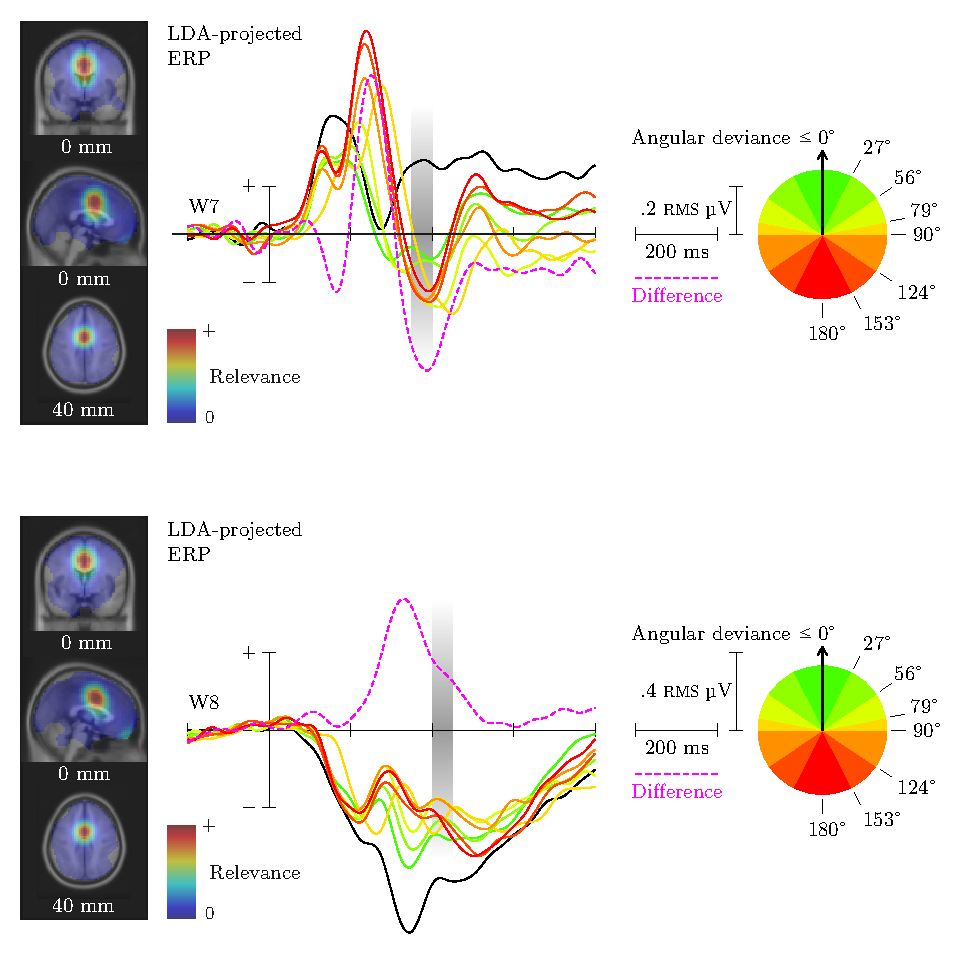
\includegraphics[width=\textwidth]{figures/nat-app-fig-s5-3.pdf}
    \caption[LDA-projected ERPs. (This figure spans three pages; this is page 1 of 3.)]{LDA-projected ERPs. (This figure spans three pages; this is page 1 of 3.) The classifier was calibrated on features spanning eight time windows of 50 ms each. For each time window, the above figures show on the left: Source localisation via weighted dipole density of the process(es) focused on in that time window; right: Full-length ERPs, combined as per that time window's LDA filter, of eight groups of cursor movement, as well as the projected difference wave between `correct' and `incorrect' classes (i.e. the filter's optimisation target). Each figure's actual time window, which actually contributed to classification, is highlighted in grey.}
\end{figure}

\begin{figure}[p]
    \renewcommand\thefigure{\ref{chapter:nat}.S6}
    \centering
    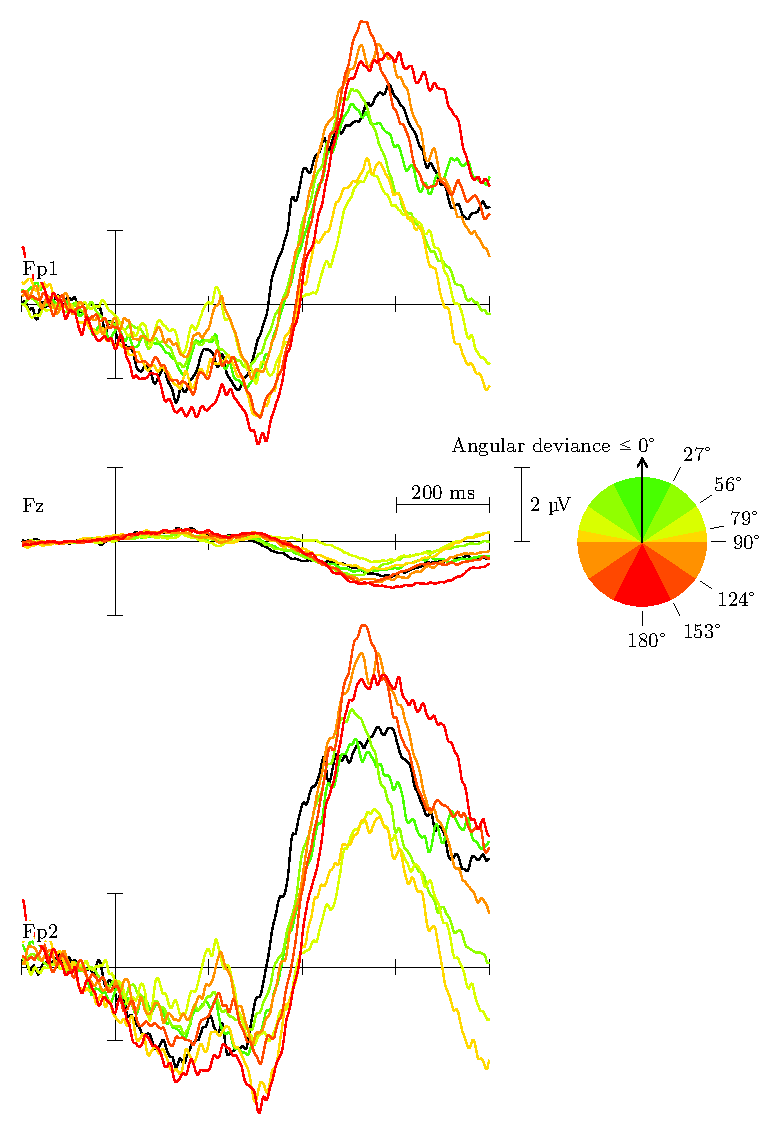
\includegraphics[width=\textwidth]{figures/nat-app-fig-s6.pdf}
    \caption[Influence of Eye Movements on the ERP at Fz.]{Influence of Eye Movements on the ERP at Fz. The grand average ERP (n = 19) at Fp1, Fp2, and Fz for only those components that contained strong eye movements and were removed for neurophysiological analysis. No systematic response is visible.}
\end{figure}

\begin{figure}[t]
    \renewcommand\thefigure{\ref{chapter:nat}.S7}
    \centering
    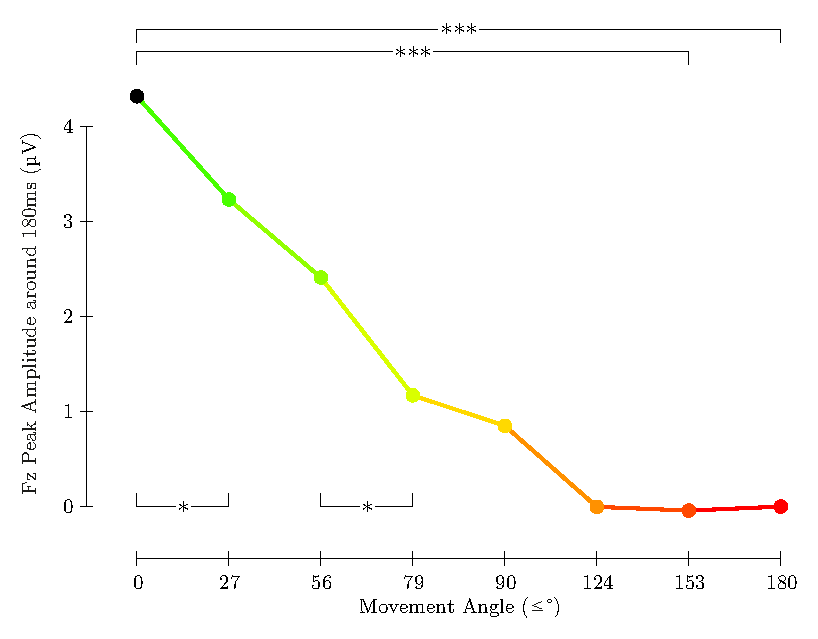
\includegraphics[scale=0.775]{figures/nat-app-fig-s7.pdf}
    \caption[Peak amplitudes around 180 ms for eight angular categories of cursor movements.]{Peak amplitudes around 180 ms for the eight groups of cursor movements. The peak amplitudes differ significantly (p < 0.001 ***) between the classes used by the classifier. In between, the peak amplitudes scale linearly with angular deviance, as fitted by a linear regression model using each group's mean angular deviance as predictor (b = -0.0035, F = 45.28, p < 0.001; R2 = 0.33). Statistically significant differences between adjacent groups are indicated as well (p < 0.05 *). See Supplementary Table S3 for exact figures of all comparisons. Classifier output followed a similar trend, as in Figure 1 of the manuscript.}
\end{figure}

\begin{figure}[b]
    \renewcommand\thefigure{\ref{chapter:nat}.S8}
    \centering
    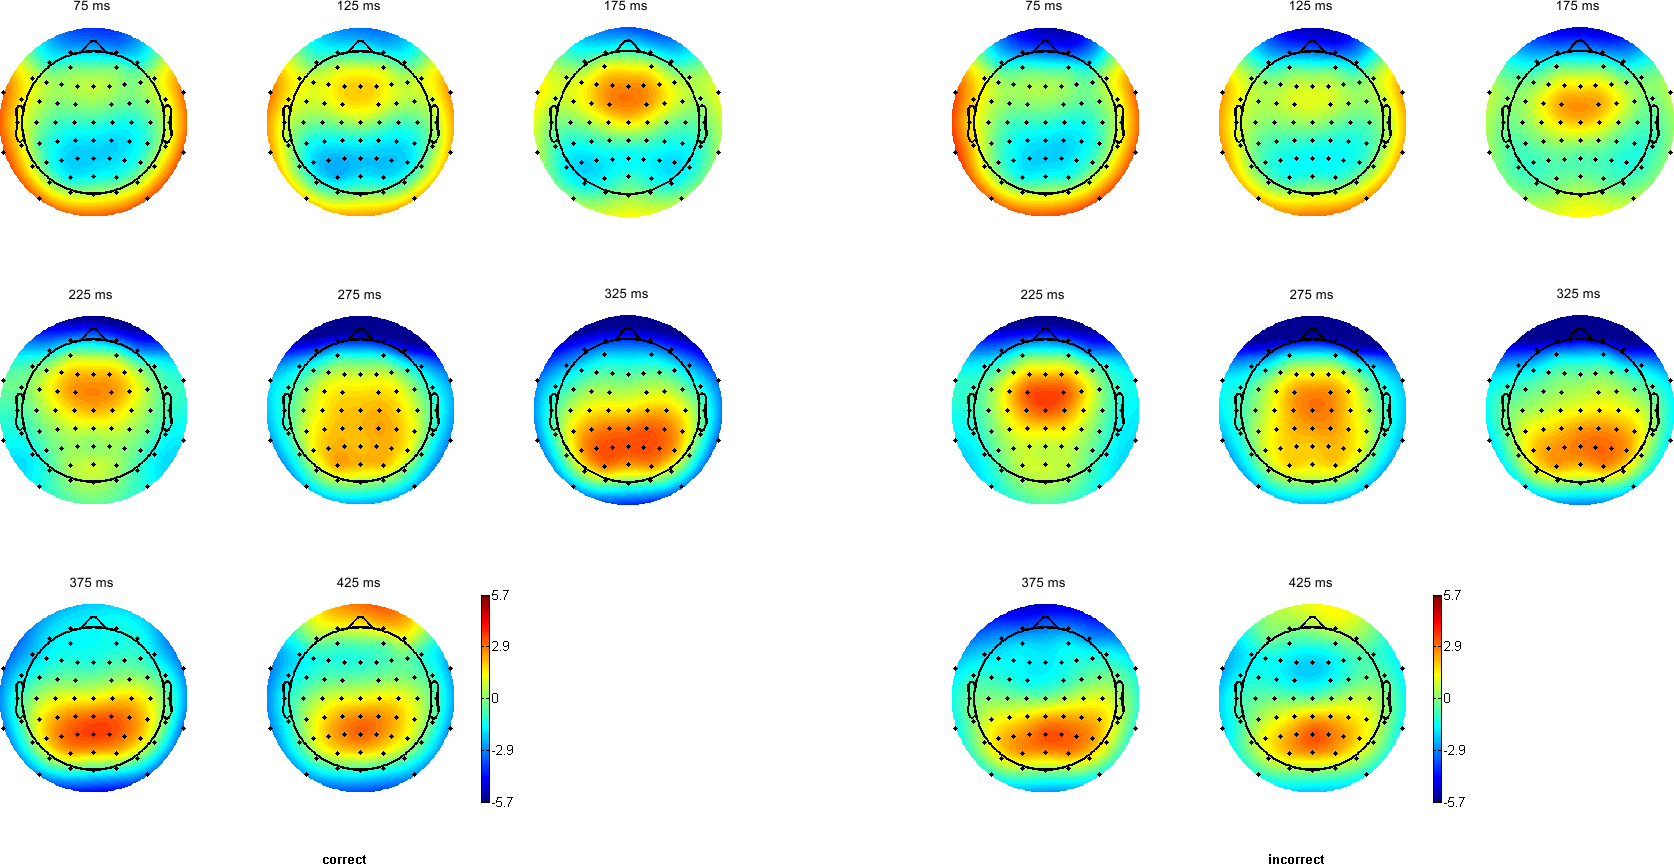
\includegraphics[width=\textwidth]{figures/nat-app-fig-s8.png}
    \caption[Scalp activity series time-locked to cursor movements.]{Scalp Activity Series. Class-specific grand average scalp activities (n = 19), time-locked to cursor movement, at the middle of each time of the eight time windows used for classification. \textit{Left:} Scalp activities of class 1, containing only cursor movements that went directly towards the target. \textit{Right:} Scalp activities of class 2, containing cursor movements with an angular deviance of 135$^\circ$ or more. EEG data was first band-pass filtered from 0.1 to 5 Hz as per the classification approach and re-referenced to the common average. See Figure 2 in the main manuscript and Supplementary Movie S1 for the class-correlated scalp activity that the classifier focused on.}
\end{figure}

\begin{figure}[p]
    \renewcommand\thefigure{\ref{chapter:nat}.S9}
    \centering
    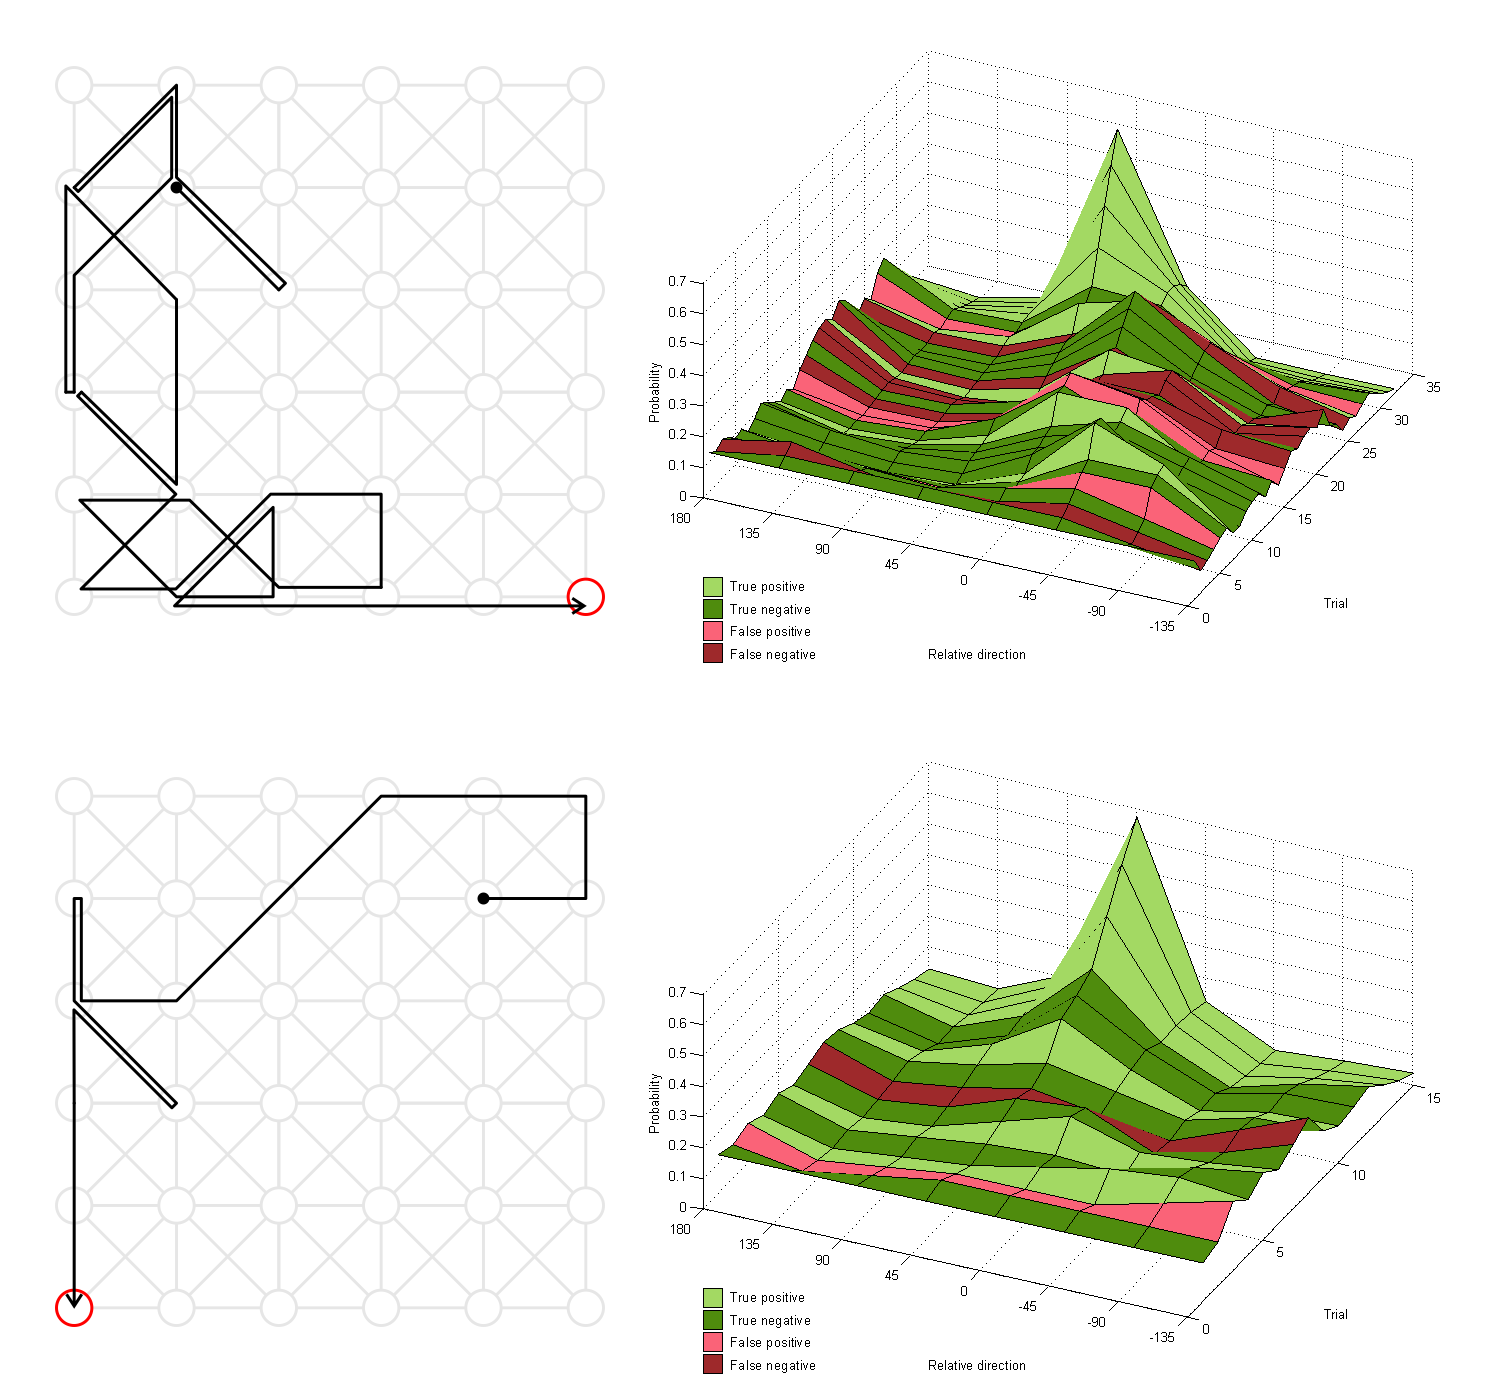
\includegraphics[width=\textwidth]{figures/nat-app-fig-s9.png}
    \caption[Example online cursor behavior.]{Example Online Cursor Behavior. Visualization of two online target selections. \textit{Left:} Trace of cursor movements over the grid. Each cursor movement only progressed one node over the grid; extended straight lines thus reflect multiple movements. \textit{Right:} Progression of normalized directional probabilities relative to 0º, with 0º being the direction towards the target at the start of the grid. All directions started out with equal probabilities, indicated at trial 0. Each subsequent trial shows the directional probabilities after that trial's cursor movement was classified and the cursor was reinforced accordingly. The colors reflect the confusion matrix with the participant's button presses being used as ground truth. True positive (light green) indicates the cursor movement was correctly classified as `correct'. True negative (dark green) indicates a correctly classified `incorrect' movement; false positive (light red) an incorrectly classified `correct' movement; false negative (dark red) an incorrectly classified `incorrect' movement. The top row shows a relatively slow online run of 31 trials on a six-by-six grid. A number of misclassifications, especially near the middle, delay the probabilistic model's convergence towards the desired target direction. However, the erroneous trials do not lead to an adverse bias while the correct classifications do systematically point towards the target, and the correct direction is found. The lower row shows a shorter run of 14 trials with only two misclassifications.}
\end{figure}

\begin{figure}[t]
    \renewcommand\thefigure{\ref{chapter:nat}.S10}
    \centering
    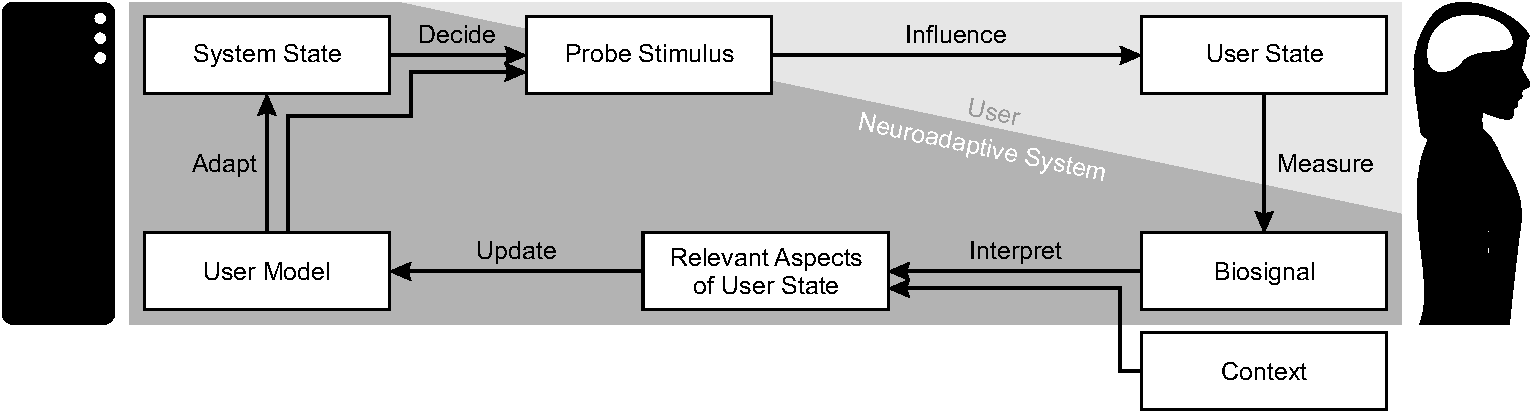
\includegraphics[width=\textwidth]{figures/nat-app-fig-s10.pdf}
    \caption[The neuroadaptive control loop.]{The neuroadaptive control loop. A stimulus or parameter change provokes an automatic response from the user, whose biosignals are monitored. The user's response can be classified from the gathered data, allowing the system to interpret the response in light of the previously gathered user information and the current context. With this information, the system updates its user model. Based on the user model and the current system status, the system may decide on a new probe stimulus.}
\end{figure}

\begin{table}[hb]
    \renewcommand\thetable{\ref{chapter:nat}.S1}
    \centering
    \small
    \begin{tabular}{ c | r r r | r r r}
        \hline \hline
        \multicolumn{1}{ c }{} & \multicolumn{3}{ c }{\textbf{4 $\times$ 4 Grids}} & \multicolumn{3}{ c }{\textbf{6 $\times$ 6 Grids}} \\
        \cline{2-7}
        Participant & TP & TN & \textbf{CR} & TP & TN & \textbf{CR} \\
        \hline \hline
        07 &  .91 & .86 & \textbf{.89} & $\cdot$ & $\cdot$ & $\cdot$ \\
        08 &  .91 & .60 & \textbf{.77} & $\cdot$ & $\cdot$ & $\cdot$ \\
        09 &  .81 & .53 & \textbf{.71} & $\cdot$ & $\cdot$ & $\cdot$ \\
        10 &  .83 & .79 & \textbf{.81} & .76 &  .75 & \textbf{.76} \\
        11 & 1.00 & .83 & \textbf{.93} & .88 & 1.00 & \textbf{.93} \\
        12 &  .83 & .63 & \textbf{.76} & .82 &  .64 & \textbf{.73} \\
        13 &  .67 & .47 & \textbf{.59} & .87 &  .38 & \textbf{.67} \\
        14 &  .75 & .63 & \textbf{.70} & .84 &  .36 & \textbf{.69} \\
        15 &  .82 & .69 & \textbf{.75} & .71 &  .82 & \textbf{.75} \\
        16 &  .52 & .50 & \textbf{.52} & .39 &  .10 & \textbf{.29} \\
        17 &  .58 & .62 & \textbf{.59} & .50 &  .68 & \textbf{.58} \\
        18 &  .67 & .62 & \textbf{.65} & .44 &  .53 & \textbf{.48} \\
        19 &  .80 & .67 & \textbf{.75} & .92 &  .65 & \textbf{.80} \\
        20 &  .71 & .80 & \textbf{.74} & .70 &  .62 & \textbf{.67} \\
        21 &  .88 & .56 & \textbf{.76} & .74 &  .45 & \textbf{.63} \\
        22 & . 60 & .67 & \textbf{.63} & .40 &  .50 & \textbf{.43} \\
        \hline \hline
        \textbf{Mean} & \textbf{.77} & \textbf{.65} & \textbf{.72} & \textbf{.69} & \textbf{.58} & \textbf{.65} \\
        \hline \hline
    \end{tabular}
    \caption[Online classification rates for cursor movements on two grid sizes.]]{Online classification rates for the 4$\times$4 grid, and the 6$\times$6  grid. TP = True Positives, TN = True Negatives, CR = Classification Rate (combined TP and TN). This table lists the classification rates for the online blocks, i.e. what percentage of classifier output agreed with the given definitions of `correct' and `incorrect' movements. These definitions were the same as the ones used for calibration: Movements with an angular deviance to the target of 0º were defined to be `correct', and those with a deviance of 135º or more were taken to be `incorrect'. The labels of all other movements were subject to individual interpretation, and have therefore not been included in this analysis. The table lists these rates for all participants that completed online blocks. From the total of nineteen, this excludes the first three participants, who only performed offline calibration blocks. A further three participants only performed 4$\times$4 grids online. }
\end{table}

\begin{table}[t]
    \renewcommand\thetable{\ref{chapter:nat}.S2}
    \centering
    \small
    \begin{tabular}{ r | r r r r r r r r }
        \hline \hline
        \multicolumn{1}{ c }{} & \multicolumn{7}{ c }{\textbf{Pairwise Comparison}} \\
        \multicolumn{1}{ c }{} & 180$^\circ$ & 135$^\circ$ & 90$^\circ$ & 45$^\circ$ & 0$^\circ$ & $-$45$^\circ$ & $-$90$^\circ$ \\
        \cline{2-8}
        135$^\circ$ & 1.000 & $\cdot$ & $\cdot$ & $\cdot$ & $\cdot$ & $\cdot$ & $\cdot$ \\
         90$^\circ$ &  0.004 & 0.003 & $\cdot$ & $\cdot$ & $\cdot$ & $\cdot$ & $\cdot$ \\
         45$^\circ$ &  0.000 & 0.000 & 0.000 & $\cdot$ & $\cdot$ & $\cdot$ & $\cdot$ \\
          0$^\circ$ &  0.000 & 0.000 & 0.000 & 1.000 & $\cdot$ &$\cdot$ & $\cdot$ \\
        $-$45$^\circ$ &  0.000 & 0.000 & 0.304 & 1.000 & 0.000 & $\cdot$ & $\cdot$ \\
        $-$90$^\circ$ &  0.000 & 0.000 & 1.000 & 0.000 & 0.000 & 0.006 & $\cdot$ \\
        $-$135$^\circ$ & 1.000 & 1.000 & 0.005 & 0.000 & 0.000 & 0.000 & 0.000 \\
        \hline \hline
    \end{tabular}
    \caption[Bonferroni-adjusted pairwise comparisons of the cursor's mean directional probabilities upon reaching the target.]{Bonferroni-adjusted pairwise comparisons of the mean directional probabilities upon reaching the target. Supplementary Figure S4 shows the mean directional probabilities upon reaching the target in both online grids, sorted by their angular deviance to the target, which was fixed relative to the cursor’s starting position. Supplementary Table S2 lists the Bonferroni-adjusted results of pairwise post-hoc tests from a one-way ANOVA (F(7,105) = 57.520, p < 0.001) on this data. On average, the classifier has been able to reinforce the ‘correct’ directions significantly more strongly than ‘incorrect’ directions.}
\end{table}

\begin{table}[b]
    \renewcommand\thetable{\ref{chapter:nat}.S3}
    \centering
    \small
    \begin{tabular}{ r | r r r r r r r r }
        \hline \hline
        \multicolumn{1}{ c }{} & \multicolumn{7}{ c }{\textbf{Pairwise Comparison}} \\
        \multicolumn{1}{ c }{} & $0^\circ$& $\leq27^\circ$ & $\leq56^\circ$ & $\leq79^\circ$ & $\leq90^\circ$ & $\leq124^\circ$ & $\leq153^\circ$ \\
        \cline{2-8}
        $\leq27^\circ$ & 0.032 & $\cdot$ & $\cdot$ & $\cdot$ & $\cdot$ & $\cdot$ & $\cdot$ \\
        $\leq56^\circ$ & 0.001 & 0.075 & $\cdot$ & $\cdot$ & $\cdot$ & $\cdot$ & $\cdot$ \\
        $\leq79^\circ$ & 0.000 & 0.000 & 0.020 & $\cdot$ & $\cdot$ & $\cdot$ & $\cdot$ \\ 
        $\leq90^\circ$ & 0.000 & 0.000 & 0.004 & 0.309 & $\cdot$ & $\cdot$ & $\cdot$ \\
        $\leq124^\circ$ & 0.000 & 0.000 & 0.000 & 0.023 & 0.071 & $\cdot$ & $\cdot$ \\
        $\leq153^\circ$ & 0.000 & 0.000 & 0.000 & 0.021 & 0.066 & 0.507 & $\cdot$ \\ 
        $\leq180^\circ$ & 0.000 & 0.000 & 0.000 & 0.023 & 0.071 & 0.520 & 0.531 \\
        \hline \hline
    \end{tabular}
    \caption[Pairwise comparisons, adjusted for false discovery rate, of the mean peak amplitudes at Fz for eight angular categories of cursor movements.]{Pairwise comparisons, adjusted for false discovery rate, of the mean peak amplitudes at Fz for the eight angular categories. A one-way ANOVA indicated a significant influence of angular deviance on peak amplitude (F(7,126) = 47.24, p < 0.001). In this table are listed the post-hoc comparisons---one-sided t-tests with pooled standard deviations, corrected for false discovery rate---between the eight individual groups of cursor movement.}
\end{table}

\clearpage

\begin{table}[t]
    \renewcommand\thetable{\ref{chapter:nat}.S4}
    \centering
    \small
    \begin{tabular}{ r | r r r r r r r r }
        \hline \hline
        \multicolumn{1}{ c }{} & \multicolumn{7}{ c }{\textbf{Pairwise Comparison}} \\
        \multicolumn{1}{ c }{} & $0^\circ$& $\leq27^\circ$ & $\leq56^\circ$ & $\leq79^\circ$ & $\leq90^\circ$ & $\leq124^\circ$ & $\leq153^\circ$ \\
        \cline{2-8}
        $\leq27^\circ$ & 0.328 & $\cdot$ & $\cdot$ & $\cdot$ & $\cdot$ & $\cdot$ & $\cdot$ \\
        $\leq56^\circ$ & 0.000 & 0.002 & $\cdot$ & $\cdot$ & $\cdot$ & $\cdot$ & $\cdot$ \\
        $\leq79^\circ$ & 0.000 & 0.000 & 0.023 & $\cdot$ & $\cdot$ & $\cdot$ & $\cdot$ \\ 
        $\leq90^\circ$ & 0.000 & 0.000 & 0.000 & 0.115 & $\cdot$ & $\cdot$ & $\cdot$ \\
        $\leq124^\circ$ & 0.000 & 0.000 & 0.000 & 0.006 & 0.125 & $\cdot$ & $\cdot$ \\
        $\leq153^\circ$ & 0.000 & 0.000 & 0.000 & 0.308 & 0.311 & 0.829 & $\cdot$ \\ 
        $\leq180^\circ$ & 0.000 & 0.000 & 0.000 & 0.311 & 0.829 & 0.979 & 0.952 \\
        \hline \hline
    \end{tabular}
    \caption[Pairwise comparisons, adjusted for false discovery rate, of the mean classifier output for eight angular categories of cursor movements.]{Pairwise comparisons, adjusted for false discovery rate, of the mean classifier output for the eight angular categories. A one-way ANOVA indicated a significant influence of angular deviance on classifier output (F(7,105) = 28.32, p < 0.001). In this table are listed the post-hoc comparisons---one-sided t-tests with pooled standard deviations, corrected for false discovery rate---between the eight individual groups of cursor movement.}
\end{table}

\begin{table}[b]
    \renewcommand\thetable{\ref{chapter:nat}.S5}
    \centering
    \small
    \begin{tabular}{ r | r r r r r r r r }
        \hline \hline
        \multicolumn{1}{ c }{} & \multicolumn{7}{ c }{\textbf{Pairwise Comparison}} \\
        \multicolumn{1}{ c }{} & $0^\circ$& $\leq27^\circ$ & $\leq56^\circ$ & $\leq79^\circ$ & $\leq90^\circ$ & $\leq124^\circ$ & $\leq153^\circ$ \\
        \cline{2-8}
        $\leq27^\circ$ & 0.004 & $\cdot$ & $\cdot$ & $\cdot$ & $\cdot$ & $\cdot$ & $\cdot$ \\
        $\leq56^\circ$ & 0.000 & 0.007 & $\cdot$ & $\cdot$ & $\cdot$ & $\cdot$ & $\cdot$ \\
        $\leq79^\circ$ & 0.000 & 0.000 & 0.009 & $\cdot$ & $\cdot$ & $\cdot$ & $\cdot$ \\ 
        $\leq90^\circ$ & 0.000 & 0.000 & 0.000 & 0.093 & $\cdot$ & $\cdot$ & $\cdot$ \\
        $\leq124^\circ$ & 0.000 & 0.000 & 0.000 & 0.168 & 0.599 & $\cdot$ & $\cdot$ \\
        $\leq153^\circ$ & 0.000 & 0.000 & 0.000 & 0.014 & 0.161 & 0.134 & $\cdot$ \\ 
        $\leq180^\circ$ & 0.000 & 0.000 & 0.000 & 0.004 & 0.046 & 0.404 & 0.227 \\
        \hline \hline
    \end{tabular}
    \caption[Pairwise comparisons of the mean amplitudes in the third time window (150-200 ms) of the LDA-projected ERP.]{Pairwise comparisons of the mean amplitudes in the third time window (150-200 ms) of the LDA-projected ERP. Supplementary Figure S5 shows LDA-projected ERPs. At Fz, significant amplitude differences were found at around 180 ms following cursor onset (see Figure 1 of the main manuscript and Supplementary Figure S7). This falls within the third time window used by the classification system (150 to 200 ms following cursor movement). This table shows the results of pairwise comparisons using one-tailed permutation tests of the mean amplitudes of the LDA-projected ERPs in that time window, between the eight individual groups of cursor movement.}
\end{table}

\begin{figure}[t]
    \renewcommand\thefigure{\ref{chapter:nat}.M1}
    \centering
    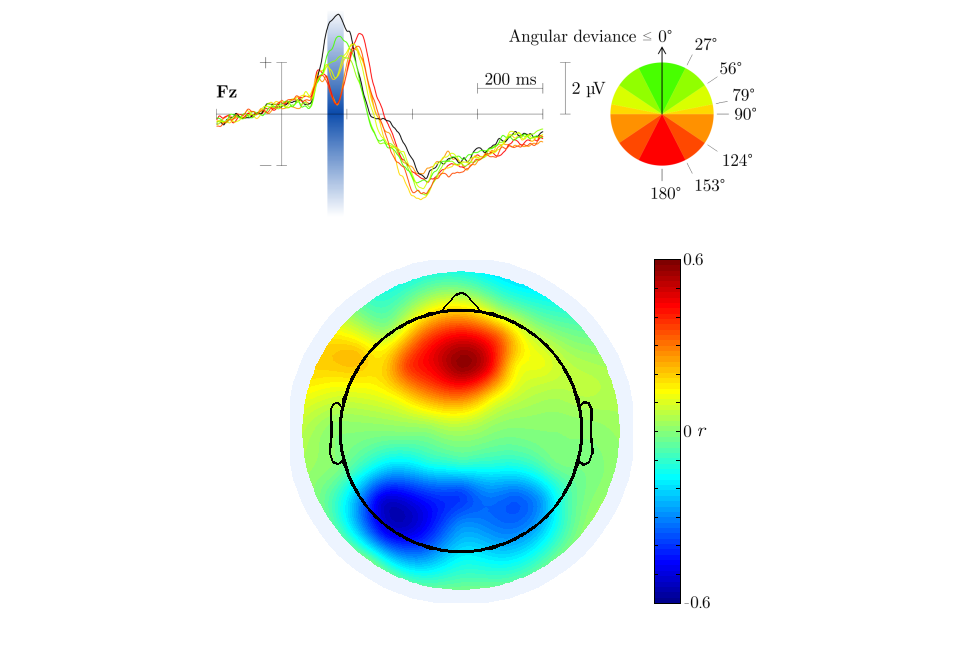
\includegraphics[width=0.9\textwidth]{figures/nat-app-movie-s1-still.png}
    \caption[Movie S1. Event-related potential at electrode Fz, and class-correlated scalp activity derived from the LDA filter weights of sequential 50-ms time windows,
spanning the 400 ms used for classification.]{Movie S1. Event-related potential at electrode Fz, and class-correlated scalp activity derived from the LDA filter weights of sequential 50-ms time windows,
spanning the 400 ms used for classification. Available online at \href{https://doi.org/10.1073/pnas.1605155114}{https://doi.org/10.1073/pnas.1605155114}}
\end{figure}

\begin{figure}[b]
    \renewcommand\thefigure{\ref{chapter:nat}.M2}
    \centering
    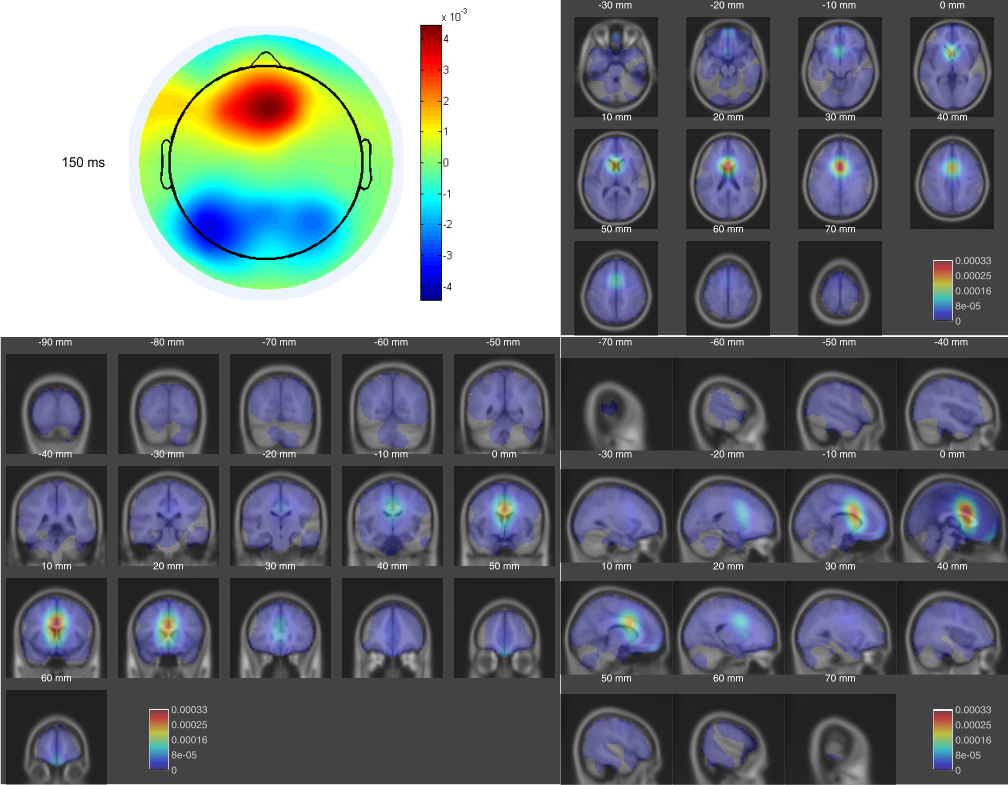
\includegraphics[width=0.8\textwidth]{figures/nat-app-movie-s2-still.png}
    \caption[Movie S2. Dipole densities weighted by relevance for classification in sequential 50-ms time windows, spanning the 400 ms used for classification.]{Movie S2. Dipole densities weighted by relevance for classification in sequential 50-ms time windows, spanning the 400 ms used for classification. Available online at \href{https://doi.org/10.1073/pnas.1605155114}{https://doi.org/10.1073/pnas.1605155114}}
\end{figure}

\begin{figure}[t]
    \renewcommand\thefigure{\ref{chapter:nat}.M3}
    \centering
    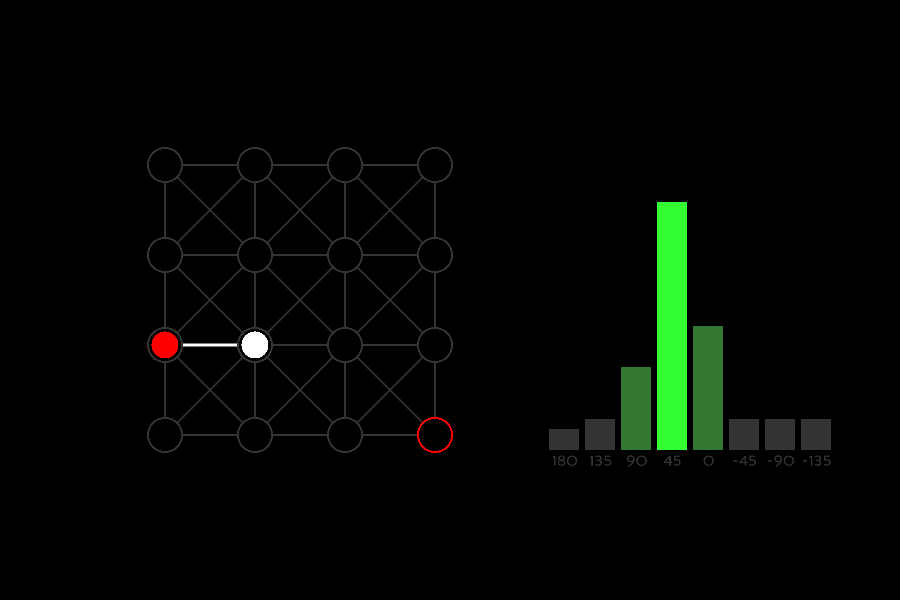
\includegraphics[width=0.9\textwidth]{figures/nat-app-movie-s3-still.png}
    \caption[Movie S3. Online experimental stimuli accompanied by classification output, illustrating the online process and outcome.]{Movie S3. Online experimental stimuli accompanied by classification output, illustrating the online process and outcome. \\ Available online at \href{https://doi.org/10.1073/pnas.1605155114}{https://doi.org/10.1073/pnas.1605155114}}
\end{figure}

\begin{figure}[b]
    \renewcommand\thefigure{\ref{chapter:nat}.M4}
    \centering
    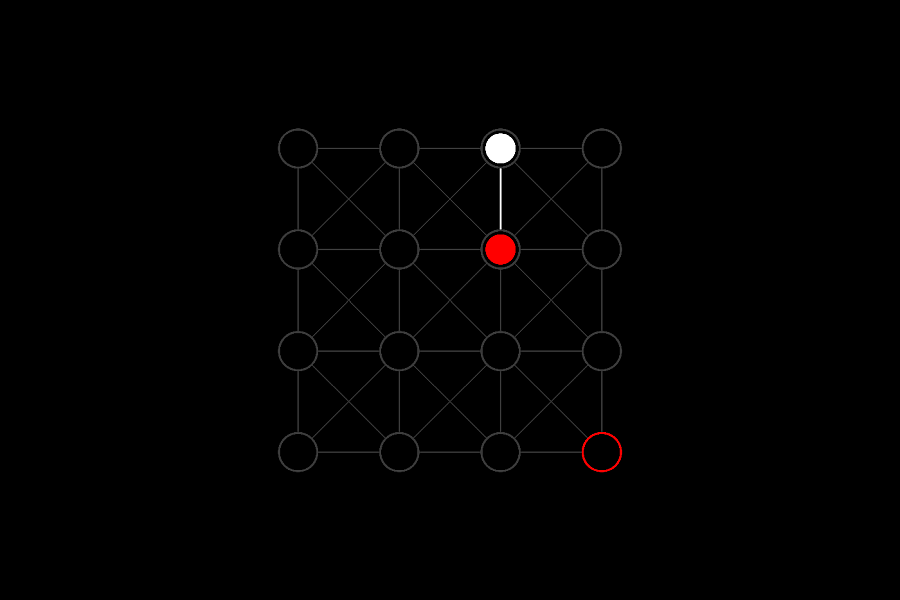
\includegraphics[width=0.9\textwidth]{figures/nat-app-movie-s4-still.png}
    \caption[Movie S4. Offline experimental stimuli.]{Movie S4. Offline experimental stimuli. \\ Available online at \href{https://doi.org/10.1073/pnas.1605155114}{https://doi.org/10.1073/pnas.1605155114}}
\end{figure}